%%%%%%%%%%%%%%%%%%%%%%%%%%%%%%%%%%%%%%%%%
% Beamer Presentation
% LaTeX Template
% Version 1.0 (10/11/12)
%
% This template has been downloaded from:
% http://www.LaTeXTemplates.com
%
% License:
% CC BY-NC-SA 3.0 (http://creativecommons.org/licenses/by-nc-sa/3.0/)
%
%%%%%%%%%%%%%%%%%%%%%%%%%%%%%%%%%%%%%%%%%

%------------------------------------------------------------------------------------------------
% PACKAGES AND THEMES
%------------------------------------------------------------------------------------------------

\documentclass[table, xcolor = {dvipsnames}, 9pt]{beamer}
\usepackage{tikz}
\usetikzlibrary{calc}
\usetikzlibrary{positioning}
\usetikzlibrary{arrows.meta}
\usetikzlibrary{external}
\mode<presentation> {

% The Beamer class comes with a number of default slide themes
% which change the colors and layouts of slides. Below this is a list
% of all the themes, uncomment each in turn to see what they look like.

\usetheme{default}
%\usetheme{AnnArbor}
%\usetheme{Antibes}
%\usetheme{Bergen}
%\usetheme{Berkeley}
%\usetheme{Berlin}
%\usetheme{Boadilla}
%\usetheme{CambridgeUS}
%\usetheme{Copenhagen}
%\usetheme{Darmstadt}
%\usetheme{Dresden}
%\usetheme{Frankfurt}
%\usetheme{Goettingen}
%\usetheme{Hannover}
%\usetheme{Ilmenau}
%\usetheme{JuanLesPins}
%\usetheme{Luebeck}
%\usetheme{Madrid}
\usetheme{metropolis}
%\usetheme{Malmoe}
%\usetheme{Marburg}
%\usetheme{Montpellier}
%\usetheme{PaloAlto}
%\usetheme{Pittsburgh}
%\usetheme{Rochester}
%\usetheme{Singapore}
%\usetheme{Szeged}
%\usetheme{Warsaw}

% As well as themes, the Beamer class has a number of color themes
% for any slide theme. Uncomment each of these in turn to see how it
% changes the colors of your current slide theme.

%\usecolortheme{albatross}
%\usecolortheme{beaver}
%\usecolortheme{beetle}
%\usecolortheme{crane}
%\usecolortheme{dolphin}
%\usecolortheme{dove}
%\usecolortheme{fly}
%\usecolortheme{lily}
%\usecolortheme{orchid}
%\usecolortheme{rose}
\usecolortheme{seagull}
%\usecolortheme{seahorse}
%\usecolortheme{whale}
%\usecolortheme{wolverine}
\usefonttheme{professionalfonts}
%\setbeamertemplate{footline} % To remove the footer line in all slides uncomment this line
%\setbeamertemplate{footline}[page number] % To replace the footer line in all slides with a simple slide count uncomment this line

%\setbeamertemplate{navigation symbols}{} % To remove the navigation symbols from the bottom of all slides uncomment this line
}

\usepackage{graphicx} % Allows including images
\usepackage{booktabs} % Allows the use of \toprule, \midrule and \bottomrule in tables
\usepackage{tikz}
\usepackage{multirow}
\usepackage{natbib}
\usepackage{hyperref}
\usepackage{diagbox}
\usepackage{makecell}
\usepackage{xparse}
\usepackage{subfig}
\usepackage{amsmath}
\usepackage{amsfonts,amsthm,amsmath,amssymb}    
\usepackage{bbm}
\usepackage{bm}
\usepackage{empheq}
\usepackage{pgfplots}
\usepackage{animate}
\usepgfplotslibrary{colorbrewer}

\newcommand\mybox[2][]{\tikz[overlay]\node[fill=lightgray,inner sep=2pt, anchor=text, rectangle, rounded corners=1mm,#1] {#2};\phantom{#2}}
\hypersetup{unicode=true,
            bookmarksnumbered=true,
            bookmarksopen=true,
            bookmarksopenlevel=2,
            breaklinks=false,
            pdfborder={0 0 1},
            hypertexnames=false,
            pdfstartview={XYZ null null 1}}
\usepackage{xcolor}
\newcommand\myheading[1]{%
  \par\bigskip
  {\Large\bfseries#1}\par\smallskip}
\newcommand\given[1][]{\:#1\vert\:}
\theoremstyle{plain}
\newtheorem{thm}{Theorem}
\newtheorem{prop}{Proposition\thisthmnumber}
\newtheorem{lem}{Lemma\thisthmnumber}
\newtheorem{cor}{Corollary}
\newtheorem{defin}{Definition}
\newtheorem{algo}{Algorithm}
\newcommand*\diff{\mathop{}\!\mathrm{d}}
\newcommand*\Diff[1]{\mathop{}\!\mathrm{d^#1}}
\newcommand{\bh}[1]{{\color{blue}{#1}}}
\newcommand{\mh}[1]{{\color{magenta}{#1}}}
\newcommand{\thisthmnumber}{}
\newcommand{\tikzmark}[1]{\tikz[baseline,remember picture] \coordinate (#1) {};}
\newcommand*{\QEDA}{\hfill\ensuremath{\blacksquare}}%
\newcommand*{\QEDB}{\hfill\ensuremath{\square}}%
\DeclareMathOperator{\E}{\rm{E}}
\DeclareMathOperator{\R}{\mathbb{R}}
\DeclareMathOperator{\N}{\mathbb{N}}
\DeclareMathOperator{\Var}{\rm{Var}}
\DeclareMathOperator{\Cov}{\rm{Cov}}
\DeclareMathOperator{\Supp}{\rm{Supp}}
\DeclareMathOperator{\e}{\rm{e}}
\DeclareMathOperator{\F}{\mathcal{F}}
\DeclareMathOperator{\Z}{\mathcal{Z}}
\DeclareMathOperator{\logit}{\rm{logit}}
\DeclareMathOperator{\indep}{{\perp\!\!\!\perp}}
\DeclareMathOperator{\rank}{rank}
\DeclareMathOperator*{\argmin}{arg\,min}
\DeclareMathOperator*{\argmax}{arg\,max}
%\DeclareMathOperator{\Pr}{\rm{Pr}}
%------------------------------------------------------------------------
% TITLE PAGE
%-----------------------------------------------------------------------
\pagestyle{empty}
\title[]{Covariance adjustment in randomized experiments} % The short title appears at the bottom of every slide, the full title is only on the title page

\author{Thomas Leavitt} % Your name
\institute[] % Your institution as it will appear on the bottom of every slide, may be shorthand to save space
{
% Your institution for the title page
\medskip
\textit{} % Your email address
}
\date{\today} % Date, can be changed to a custom date

\begin{document}

\begin{frame}
\titlepage % Print the title page as the first slide
\end{frame}

%\begin{frame}
%\frametitle{Overview} % Table of contents slide, comment this block out to remove it
%\tableofcontents % Throughout your presentation, if you choose to use \section{} and \subsection{} commands, these will automatically be printed on this slide as an overview of your presentation
%\end{frame}

%------------------------------------------------------------------------
% PRESENTATION SLIDES
%------------------------------------------------------------------------
\begin{frame}{Covariance adjustment in randomized experiments: Introduction}
\vfill
\begin{itemize}
\item We often have information contained in baseline covariates\pause \vfill
\begin{itemize} \vfill
\item I.e., variables measured \textbf{prior} to treatment assignment \pause \vfill
\end{itemize} \vfill
\item If baseline covariates related to POs, we want to use covariates to increase\vfill
\begin{enumerate}
\item precision of our estimators and \vfill 
\item power of our tests \vfill
\end{enumerate} \vfill
\end{itemize} \vfill
\end{frame}
%------------------------------------------------------------------------
\begin{frame}{Covariance adjustment in randomized experiments: Introduction}
\vfill
\begin{itemize}
\item Two primary approaches to covariance adjustment we will cover \pause \vfill
\begin{enumerate} \vfill
\item Random assignment within blocks of units similar in covariates \pause \vfill
\item Rescaling outcomes to make their variance smaller  \vfill
\end{enumerate}  \vfill
\end{itemize} \vfill
\end{frame}
%------------------------------------------------------------------------
\section{Block random assignment}
\begin{frame}{Block random assignment}
\vfill
\begin{itemize} \vfill
\item Construct blocks of units similar in baseline covariates related to POs \vfill
\item By blocking we reduce number of possible assignments \vfill
\item Goal is to exclude assignments that yield estimates far from truth \\ so that estimator will be closer to truth, on average \vfill
\end{itemize} \vfill
\end{frame}
%------------------------------------------------------------------------
\begin{frame}{Block random assignment: Example}
\vfill
\bh{Example}: Experiment with $N = 6$ units, $n_T = 3$ and $n_C = 3$
\begin{table}[H]
\centering{}
    \begin{tabular}{l|l|l|l}
    $\bm{y_C}$ & $\bm{y_T}$ & $\bm{\tau}$ & $\bm{x}$ \\ \hline
  20 & 22 & 2 & 1 \\
  8 & 12 & 4 & 1 \\
  11 & 11 & 0 & 0 \\
  10 & 15 & 5 & 1 \\
  14 & 18 & 4 & 1 \\
  1 &  4 & 3 & 0 \\
    \end{tabular}
\caption{True values of $\bm{y_C}$, $\bm{y_T}$, $\bm{\tau}$ and baseline covariate $\bm{x}$}
\end{table} \vfill
Stratify on $\bm{x}$ and assign half of units to treatment within strata \vfill

In this case, instead of $\binom{6}{3} = 20$ assignments, we have $\prod \limits_{b = 1}^B \binom{N_b}{n_{Tb}} = 12$ assignments, where $b = 1, \ldots , B$ indexes the blocks \vfill
\end{frame}
%------------------------------------------------------------------------
\begin{frame}{Block random assignment: Example}
\vfill
\begin{itemize} \vfill
\item Here is set of assignments in this example under block random assignment \vfill
\item Units with \mh{$x_i = 1$}; units with \bh{$x_i = 0$} \vfill
\end{itemize} 
\vfill
\begin{equation*}
\Omega =
\left\{
\begin{bmatrix} \mh{1} \\ \mh{1} \\ \bh{1} \\ \mh{0} \\ \mh{0} \\ \bh{0} \end{bmatrix},
\begin{bmatrix} \mh{1} \\ \mh{1} \\ \bh{0} \\ \mh{0} \\ \mh{0} \\ \bh{1} \end{bmatrix},
\begin{bmatrix} \mh{1} \\ \mh{0} \\ \bh{1} \\ \mh{1} \\ \mh{0} \\ \bh{0} \end{bmatrix},
\begin{bmatrix} \mh{1} \\ \mh{0} \\ \bh{1} \\ \mh{0} \\ \mh{1} \\ \bh{0} \end{bmatrix},
\begin{bmatrix} \mh{1} \\ \mh{0} \\ \bh{0} \\ \mh{1} \\ \mh{0} \\ \bh{1} \end{bmatrix},
\begin{bmatrix} \mh{1} \\ \mh{0} \\ \bh{0} \\ \mh{0} \\ \mh{1} \\ \bh{1} \end{bmatrix},
\begin{bmatrix} \mh{0} \\ \mh{1} \\ \bh{1} \\ \mh{1} \\ \mh{0} \\ \bh{0} \end{bmatrix},
\begin{bmatrix} \mh{0} \\ \mh{1} \\ \bh{1} \\ \mh{0} \\ \mh{1} \\ \bh{0} \end{bmatrix},
\begin{bmatrix} \mh{0} \\ \mh{1} \\ \bh{0} \\ \mh{1} \\ \mh{0} \\ \bh{1} \end{bmatrix},
\begin{bmatrix} \mh{0} \\ \mh{1} \\ \bh{0} \\ \mh{0} \\ \mh{1} \\ \bh{1} \end{bmatrix},
\begin{bmatrix} \mh{0} \\ \mh{0} \\ \bh{1} \\ \mh{1} \\ \mh{1} \\ \bh{0} \end{bmatrix},
\begin{bmatrix} \mh{0} \\ \mh{0} \\ \bh{0} \\ \mh{1} \\ \mh{1} \\ \bh{1} \end{bmatrix}
\right\}.
\label{eq: example block omega}
\end{equation*}
\vfill
\begin{itemize}
\item There are only $12$ assignments (instead of 20) because we have the constraint that exactly half of units with $\mh{x_i = 1}$ have to be treated and half of units with $\bh{x_i = 0}$ have to be treated
\end{itemize}
\end{frame}%------------------------------------------------------------------------
\begin{frame}{Block random assignment: Example}
\begin{figure}[H]
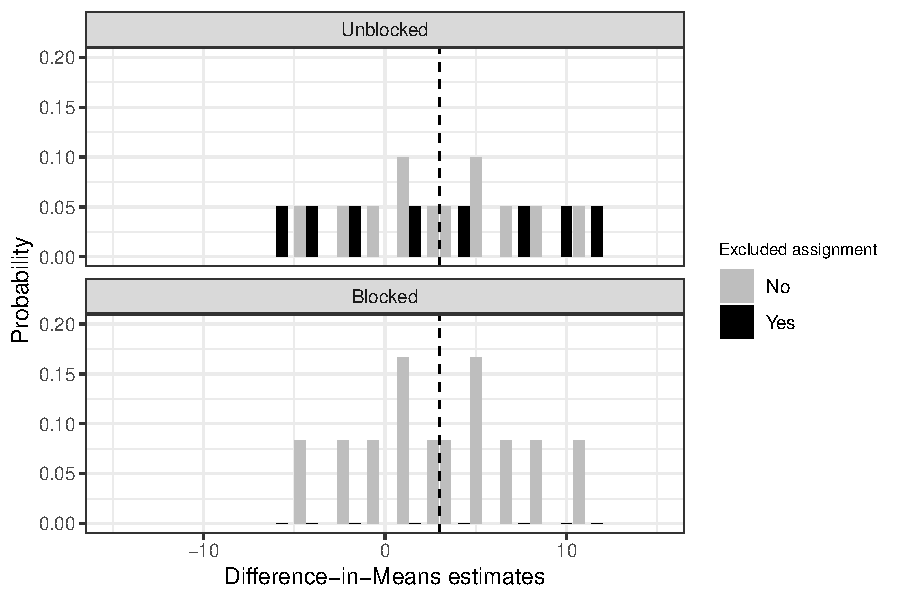
\includegraphics[width=0.9\linewidth]{blocked_assign_plot.pdf}
\caption{Difference-in-Means distribution under unblocked and blocked assignment}
\end{figure}
\end{frame}%------------------------------------------------------------------------
\section{Rescaling outcomes}
\begin{frame}{Rescaling outcomes}
\vfill
\begin{itemize} \vfill
\item For example, let's go back to expression for variance of Diff-in-Means \vfill
\begin{equation*}
\Var\left[\hat{\tau}\left(\bm{Z}, \bm{Y}\right)\right] = \frac{1}{N - 1}\left(\frac{n_T \mh{\sigma^2_{y_C}}}{n_C} + \frac{n_C \mh{\sigma^2_{y_T}}}{n_T} + 2\mh{\sigma_{y_C, y_T}}\right)
\end{equation*} \vfill
\item Can we rescale outcomes so that $\mh{\sigma^2_{y_C}}$ and $\mh{\sigma^2_{y_T}}$ are smaller? \pause \vfill
\item Importantly, such rescaling cannot alter individual treatment effects: 
\begin{align*}
y_{Ti} - x_i - \left(y_{Ci} - x_i\right) = y_{Ti} - x_i - y_{Ci} + x_i = y_{Ti} - y_{Ci}
\end{align*}
or the average treatment effect \pause \vfill
\item $x_i$ could be outcome from prior time period (gain scores) \vfill
\item Could also be predictions of a model, $y_{Ti} - f(x_i) - \left(y_{Ci} - f(x_i)\right)$ (Rosenbaum 2002) \vfill
\item Ideally, model fit to historical data or set-aside sample not in experiment \vfill
\end{itemize} \vfill
\end{frame}
%------------------------------------------------------------------------
\begin{frame}{Rescaling outcomes}
\vfill
\begin{itemize} \vfill
\item \bh{Example}: Acorn GOTV experiment (Arceneaux, 2005):
\end{itemize} 
\begin{center}
  \begin{tabular}{r|rrr}
  \hline
 & GOTV? & vote03(\%) & vote03 - vote02(\%) \\
  \hline
1 & 0 & 38 & -36 \\
$\vdots$& $\vdots$& $\vdots$ & $\vdots$ \\
13 & 0 & 19 & -38 \\
14 & 0 & 34 & -27 \\
15 & 1 & 49 & -25 \\
16 & 1 & 38 & -28 \\
$\vdots$& $\vdots$& $\vdots$ & \\
28 & 1 & 29 & -32\\
   \hline
\end{tabular}
\end{center} \vfill
Now conduct analysis on rescaled vote03 - vote02(\%) outcome
\end{frame}
%------------------------------------------------------------------------
\begin{frame}{Rescaling outcomes} \vfill
Here is distribution of Diff-in-Means for test of sharp null of no effects using original outcome and gain-score outcome
\begin{figure}[H]
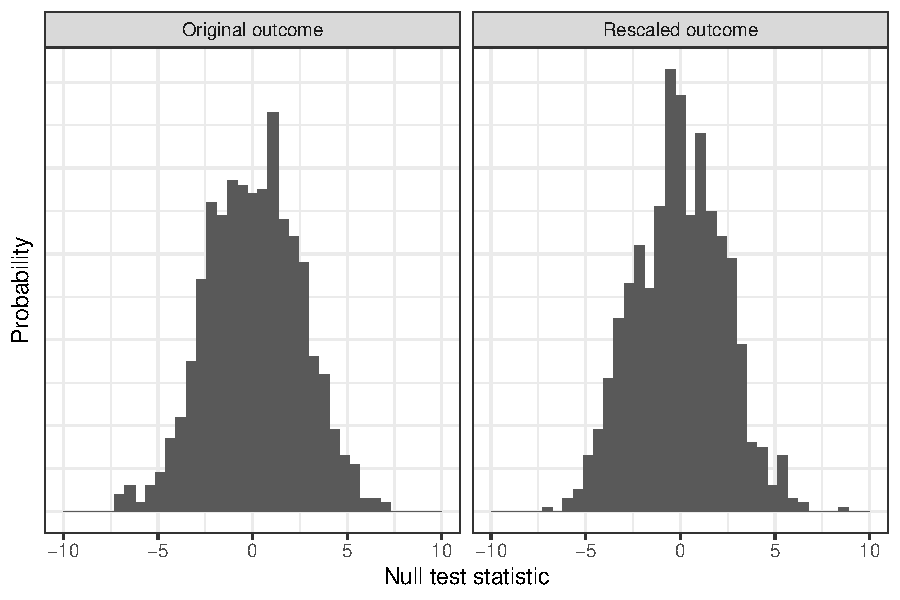
\includegraphics[width=0.9\linewidth]{null_dist_no_effect_plot.pdf}
\caption{Difference-in-Means under sharp null on original and rescaled outcomes}
\end{figure}
\end{frame}
%------------------------------------------------------------------------
\end{document}